\documentclass[a4paper,12pt,twoside]{ThesisStyle}
\usepackage[utf8]{inputenc}
\usepackage{thesis-style}
\usepackage[catalan]{babel}

\begin{document}

\frontmatter

\pagenumbering{gobble}

\thispagestyle{empty}
\begin{table}[htb]
\centering
\begin{Large}
\resizebox{\textwidth}{!}{\begin{tabular}{ | l |}
 \hline
 \\

\includegraphics[scale=0.9]{imatges/logo_eps.png} \\[0.7cm]
\centerline{Treball Final de Màster}\\[1cm]
\hline
\\
Estudi: Màster en Ciència de Dades\\[0.7cm]
\hline
\\
Títol: Resolució del Travelling Salesman Problem (TSP) mitjançant Xarxes Neuronals.\\[0.7cm]
\hline
\\
Document: Memòria\\[0.7cm]
\hline
\\
Alumne: Enric Piñera i Pons\\[0.7cm]
\hline
\\
Tutor: Josep Suy Franch\\
Departament:\\
Àrea:\\[0.7cm]
\hline
\\
Convocatòria (mes/any): Juny 2026\\[0.7cm]
\hline

\end{tabular}}
\end{Large}
\end{table}

\newpage
\hypersetup{pageanchor=false}
\begin{titlepage}

% Upper part of the page

\includegraphics[scale=0.9]{imatges/logo_eps.png} \\[1cm]
\begin{center}
\textsc{\Large Treball Final de Màster} \\[1cm]

% Title
\begin{spacing}{2}
\HRule \\
\textbf{\Huge Resolució del Traveling Salesman Problem (TSP) utilitzant Xarxes Neuronals} \\
\HRule \\[0.5cm]
\end{spacing}

% Author and supervisor and other data
{
\large
\emph{Autor:} \\
Enric \textsc{Piñera i Pons} \\[1cm]
Juny 2025 \\[1cm]
Màster en Ciència de Dades \\[1cm]
\emph{Tutors:} \\
Josep \textsc{Suy Franch} \\
Nom \textsc{Cognoms} \\
}

\end{center}
\end{titlepage}
\hypersetup{pageanchor=true}

\titlepage

%\dominitoc


\pagenumbering{roman}

\chapter*{Resum}
%\label{cap:resum}



\chapter*{Agraïments}
%\label{cap:agraiments}

Per començar vull agrair molt especialment a \ldots


\tableofcontents

\listoffigures

\listoftables

\mainmatter


\chapter{Introducció}
\label{cap:intro}

\section{Presentació del problema}
\label{PresentacioProblema}

El Traveling Salesman Problem (TSP) és un problema clàssic en la teoria d'optimització combinatòria.  
Va ser estudiat al segle XVIII pels matemàtics Sir William Rowan Hamilton, irlandès, i Thomas Penyngton Kirkman, britànic. Es creu que la seva formulació general va ser estudiada per primer cop per Karl Menger a Viena i Harvard.

\medskip

El TSP consisteix a trobar el recorregut més curt per a un viatjant que ha de visitar un conjunt de ciutats, passant per cadascuna exactament una vegada i tornant a la ciutat d'origen.

\medskip

Aquest problema és NP-complet, cosa que implica que no existeix un algorisme que el resolgui eficientment en tots els casos, especialment quan el nombre de ciutats és gran. De fet, sigui \( n \) el nombre de ciutats a visitar, el nombre total de possibles rutes que cobreixen totes les ciutats es pot expressar com el conjunt de solucions factibles del problema i està donat per \( \frac{(n-1)!}{2} \).

\medskip

A grans trets, el TSP es classifica com symmetric travelling salesman problem (sTSP), asymmetric travelling salesman problem (aTSP), and multi travelling salesman problem (mTSP):
\begin{itemize}
  \item \textbf{TSP simètric (sTSP):} Sigui \( V = \{ v_1, \dots, v_n \} \) un conjunt de ciutats, \( A = \{ (r,s) : r,s \in V \} \) el conjunt d'arestes, i \( d_{rs} = d_{sr} \) una mesura de cost associada a l'aresta \( (r,s) \in A \). El sTSP consisteix a trobar una ruta tancada de longitud mínima que visiti cada ciutat una sola vegada. En aquest cas, si les ciutats \( v_i \in V \) estan representades per les seves coordenades \( (x_i, y_i) \) i \( d_{rs} \) és la distància euclidiana entre \( r \) i \( s \), llavors tenim un Euclidean TSP.
  \item \textbf{TSP asimètric (aTSP):} Si \( d_{rs} \neq d_{sr} \) per almenys una parella \( (r,s) \), llavors el problema esdevé un aTSP.
  \item \textbf{TSP amb múltiples venedors (mTSP):} Es defineix com un conjunt de vèrtexs en què hi ha \( m \) venedors situats en un únic depòsit. La resta de vèrtexs (ciutats) són vèrtexs intermedis que cal visitar. L'objectiu és trobar rutes per als \( m \) venedors, assegurant que tots comencin i acabin al depòsit, que cada ciutat sigui visitada exactament una vegada, i que el cost total sigui mínim. Aquesta variant pot incloure restriccions addicionals com la capacitat dels venedors o horaris de visita.
\end{itemize}

\medskip

Aquest treball es centra en la resolució del TSP simètric euclidià, per la seva simplicitat i la reducció significativa pel que fa al cost computacional. No obstant això, les tècniques desenvolupades en aquest treball poden servir com a base per a abordar les variants asimètriques i de múltiples venedors del TSP en futurs treballs.


\section{Aplicacions}
\label{Aplicacions}

Més enllà de l'interès purament teòric que té la investigació dels diferents mètodes de resolució del TSP, aquest problema apareix en una gran varietat d'aplicacions pràctiques. El TSP apareix de manera natural i directa en problemes de transport o logística, com podria ser la ruta que fa un autobús escolar o el transport de mercaderies. De fet, aquestes qüestions ja van motivar les primeres investigacions sobre el TSP als anys 40. Tanmateix, també apareix en àmbits no tan intuïtius com els que es descriuen a continuació:

\subsection{Perforació de plaques de circuits impresos}

Una aplicació directa del TSP és el problema de perforació de plaques de circuits impresos (PCB) \cite{grotschel1991drilling}. Per connectar un conductor d'una capa amb un conductor d'una altra capa, o per posicionar els pins dels circuits integrats, s'han de perforar forats a través de la placa. Els forats poden ser de diferents mides. Per perforar consecutivament dos forats de diàmetres diferents, el capçal de la màquina s'ha de moure fins a una caixa d'eines i canviar l'eina de perforació. Això requereix força temps. Per tant, és clar que cal triar un diàmetre, perforar tots els forats del mateix diàmetre, canviar el trepant, perforar els forats del següent diàmetre, etc.

Així, aquest problema de perforació es pot veure com una sèrie de TSP, un per a cada diàmetre de forat, on les ``ciutats'' són la posició inicial i el conjunt de tots els forats que es poden perforar amb el mateix trepant. La ``distància'' entre dues ciutats ve donada pel temps que es triga a moure el capçal de perforació d'una posició a l'altra. L'objectiu és minimitzar el temps de desplaçament del capçal de la màquina.

\subsection{Revisió de turbines de gas}

Una altra aplicació del TSP es troba en el manteniment i revisió de turbines de gas en motors d'aeronaus \cite{plante1987product}. Per tal de garantir un flux de gas uniforme a través de les turbines, hi ha conjunts de pales guia (nozzle-guide vane assemblies) situats a cada etapa de la turbina. Aquests conjunts consisteixen en un nombre de pales disposades al llarg de la seva circumferència, cadascuna amb característiques individuals.

La disposició adequada d'aquestes pales pot comportar beneficis significatius, com ara la reducció de vibracions, una major uniformitat del flux i una disminució del consum de combustible. El problema de determinar l'ordre òptim de col·locació de les pales es pot modelitzar com un TSP amb una funció objectiu especial.

\subsection{Cristal·lografia de raigs X}

L'anàlisi de l'estructura de materials cristal·lins mitjançant tècniques de difracció de raigs X constitueix una altra aplicació rellevant del TSP \cite{bland1989large}. En aquest context, un difractòmetre de raigs X s'utilitza per obtenir informació sobre l'estructura interna del material. Per fer-ho, un detector mesura la intensitat de les reflexions de raigs X des de diferents posicions.

Tot i que cada mesura es pot realitzar ràpidament, el temps necessari per posicionar el dispositiu és considerable, especialment quan cal visitar centenars de milers de posicions. El temps de desplaçament entre dues posicions es pot calcular amb gran precisió, i el resultat final de l'experiment no depèn de l'ordre en què es realitzen les mesures. Tanmateix, el temps total sí que en depèn. Per aquest motiu, el problema consisteix a trobar una seqüència de posicions que minimitzi el temps total de desplaçament.

\subsection{Aplicacions en genòmica i bioinformàtica}

El TSP també té aplicacions en l'àmbit de la genòmica, especialment en la construcció de mapes genètics i en problemes de seqüenciació. En aquests contextos, sovint es disposa d'un conjunt de fragments o mapes locals que s'han d'integrar en una única estructura coherent. Aquest problema es pot modelitzar com un TSP en què les ``ciutats'' representen els fragments, i el cost de desplaçament entre dos elements reflecteix la probabilitat o qualitat de la seva adjacència \cite{agarwala2000radiation, stewart2001mouse}.

A més, problemes relacionats amb la reconstrucció de seqüències d'ADN també es poden formular en termes del TSP. En aquest cas, es considera un conjunt de cadenes d'ADN de longitud fixa que s'han d'integrar en una seqüència global més curta possible. El cost entre dues cadenes es defineix en funció del solapament màxim entre elles, i l'objectiu és trobar un ordre que minimitzi la longitud total de la seqüència resultant \cite{pevzner2000computational}.

\subsection{Planificació d'observacions astronòmiques}

En l'àmbit de l'enginyeria espacial, el TSP s'ha utilitzat per optimitzar la seqüència d'observació d'objectes celestes en missions amb satèl·lits. En aquest cas, les ``ciutats'' corresponen als objectes a observar, i el cost de desplaçament representa el combustible necessari per reorientar els satèl·lits entre observacions consecutives \cite{spears2000fuel}.

L'objectiu és determinar l'ordre d'observació que minimitzi el consum total de combustible, fet que pot tenir un impacte significatiu en la viabilitat i durada de la missió.


\section{Motivació}
\label{Motivació}

En els últims anys s'ha produït un gran avenç en el camp de les xarxes neuronals. Les altes capacitats computacionals dels dispositius actuals permeten entrenar models de \textit{machine learning} amb unes limitacions molt menys restrictives que les que hi havia fa només uns anys i, per tant, s'han pogut posar en pràctica models teòrics que ja existien des de fa dècades i que només s'havien aplicat amb un nombre molt petit de paràmetres a causa de les limitacions computacionals.

\medskip

Aquest treball té com a objectiu proposar una nova manera de resoldre el TSP, aprofitant precisament els avenços en computació i \textit{machine learning} dels últims anys. En particular, es planteja dissenyar i entrenar una Xarxa Neuronal de Gràfics (GNN) i/o un Transformer capaç de resoldre el problema del TSP de manera eficient i competitiva en comparació amb els heurístics clàssics.

\medskip

Com ja s'ha comentat anteriorment, el TSP és un problema NP-complet. Això implica que, tot i que existeixen algoritmes per trobar la solució òptima, el temps computacional necessari és molt elevat i sovint inassumible en escenaris on cal obtenir solucions en un temps raonable o en problemes amb varis milers de ciutats.

\medskip

S'han dedicat molts anys de recerca a desenvolupar algoritmes heurístics que, tot i no garantir una solució òptima, ofereixen solucions de bona qualitat en un temps computacional raonable. En aquest context, aquest treball se centra en el desenvolupament d'un nou heurístic i en la seva comparació, tant en qualitat de la solució com en temps computacional, amb alguns dels heurístics clàssics més coneguts.

\medskip

Aquesta nova manera de resoldre el TSP mitjançant xarxes neuronals proporciona un enfocament completament diferent del dels heurístics clàssics. En aquest nou escenari, el temps computacional no depèn directament dels paràmetres del graf, sinó del temps que triga el model a fer una predicció; és a dir, del temps necessari per propagar la informació del graf a través dels pesos i transformacions pròpies de la xarxa neuronal. Així, el temps d'inferència s'espera que sigui significativament inferior al dels heurístics clàssics. En contraposició, el cost computacional principal es concentra en el procés d'entrenament del model, que es duu a terme prèviament. Aquest procés requereix, en efecte, un temps computacional molt més elevat que el dels heurístics clàssics. Tanmateix, es pot considerar com un cost fix que s'assumeix una sola vegada i que posteriorment permet obtenir solucions de manera molt ràpida.

Perquè es important avui en dia?
Es compara heuristics vs xxnn, cal explicar per sobre què es diferencien i perquè és interessant comparar-los.
Quins beneficis podria tenir utilitzar una xxnn?
Quins són els treballs similars que hi ha a la literatura i/o quina literatura ha servit de base per a desenvolupar el treball?
Si hi ha treballs similars, que diferencia aquest treball dels ja existents?
Quines són les contribucions més importants del treball (e.g., recopilació de dades, desenvolupament de mètodes i algorismes, experiments, representació de la informació obtinguda, ...)?



\section{Resultats}
\label{Resultats}




























\chapter{Estat de l'art}
\label{cap:estat}

\section{Investigació i anàlisi de les diferents heurístiques existents}
\label{SolucionsClassiques}
Hi ha principalment dues maneres de resoldre el TSP de manera òptima. La primera és aplicar un enfocament exacte com el mètode de Branch and Bound per trobar la longitud. L'altra és calcular el límit inferior de Held-Karp, que produeix un límit inferior per a la solució òptima. Aquest límit inferior s'utilitza per jutjar el rendiment de qualsevol nova heurística proposada per al TSP. Les heurístiques descrites en aquest treball es refereixen al sTSP, però es poden modificar adequadament per resoldre el aTSP.

\medskip

Resoldre el TSP de manera òptima, fins i tot per a casos de mida moderada, requereix un temps computacional molt gran, per tant, existeix espai per al desenvolupament i l'aplicació d'algorismes aproximats o heurístics. L'enfocament aproximat mai garanteix una solució òptima, però ofereix una solució gairebé òptima amb un esforç computacional raonable. Fins ara, l'algorisme aproximat més conegut és el de (Arora, 1998) amb una complexitat \( O \left( n \left( log_2 n \right) ^{O(c)} \right) \), on \( n \) és la mida del problema del TSP.

\subsection{Algorismes heurístics de construcció de circuits}
\label{AlgorismesHeuristicsConstruccio}
Tots els algorismes heurístics de construcció de circuits s'aturen quan es troba una solució i mai intenten millorar-la. Es creu que aquests algorismes troben solucions dins d'un marge del 10-15\% de l'òptim. A continuació es descriuen alguns dels algorismes heurístics de construcció de circuits disponibles a la literatura publicada.

\subsubsection{Closest neighbor}
\label{ClosestNeighbor}
Aquest és l'heurística més senzilla i directa per al TSP. La clau d'aquest enfocament és sempre visitar la ciutat més propera. La complexitat polinòmica associada amb aquesta algorisme és \( O(n^2) \). El Closest neighbor és molt similar a l'algorisme del minimum spanning tree. Els passos del Closest neighbor són els següents:
\begin{enumerate}
  \item Selecciona una ciutat aleatòria.
  \item Troba la ciutat no visitada més propera i ves-hi.
  \item Queden ciutats no visitades? Si és així torna al pas 2.
  \item Torna a la primera ciutat.
\end{enumerate}
El Closest Neighbot generalment manté el circuit dins del 25\% del límit inferior de Held-Karp (Johnson \& McGeoch, 1995).

\subsubsection{Greedy}
\label{Greedy}
Aquesta heurística construeix gradualment un circuit seleccionant repetidament l'aresta més curta i afegint-la al circuit sempre que no creï un cicle amb menys de \( N \) arestes, ni augmenti el grau de cap vèrtex a més de 2. Naturalment, no s'ha d'afegir la mateixa aresta dues vegades. La complexitat de l'algorisme és \( O(n^2) \). Els passos del Greedy són els següents:
\begin{enumerate}
  \item Ordenar totes les arestes.
  \item Seleccionar l'aresta més curta i afegir-la al nostre circuit si no viola cap de les condicions esmentades anteriorment.
  \item Tenim \( N \) arestes al nostre circuit? Si NO és així torna al pas 2.
\end{enumerate}
L'algorisme Greedy normalment manté la solució dins del 15-20\% del límit inferior de Held-Karp (Johnson \& McGeoch, 1995).


\subsection{Algorismes heurístics de millora de circuits}
\label{AlgorismesHeuristicsMillora}
Després de generar el circuit mitjançant qualsevol algorisme heurístic de construcció de circuits, es pot aplicar un algorisme heurístic de millora de circuits per millorar la qualitat del circuit generat. Popularment, es fa servir l'heurístic de 2-opt o 3-opt.

\subsubsection{2-opt i 3-opt}
\label{2opt3opt}
L'algorisme 2-opt elimina dues arestes de manera aleatòria del circuit ja generat i reconnecta els dos nous camins creats. Això es coneix com un moviment 2-opt. La reconnexió es fa de manera que es mantingui el circuit vàlid (vegeu la Figura~\ref{fig:2opt3opt} (a)). Això es fa només si el nou circuit és més curt que l'anterior. Aquest procés es continua fins que no sigui possible cap més millora. El circuit resultant és ara 2-optimal. L'algorisme 3-opt funciona de manera similar, però en lloc d'eliminar dues arestes, n'elimina tres. Això vol dir que hi ha dues maneres de reconnectar els tres camins en un circuit vàlid (vegeu la Figura~\ref{fig:2opt3opt} (b) i la Figura~\ref{fig:2opt3opt} (c)). La cerca es completa quan no es poden fer més moviments 3-opt per millorar la qualitat del circuit. Si un circuit és 3-optimal també és 2-optimal (Helsgaun). Fer el moviment 2-opt sovint dóna lloc a un circuit amb una longitud inferior al 5\% per sobre del límit de Held-Karp. Les millores d'un moviment 3-opt generalment generen un circuit aproximadament un 3\% per sobre del límit de Held-Karp (Johnson \& McGeoch, 1995).
\begin{figure}[htb]
  \centering
  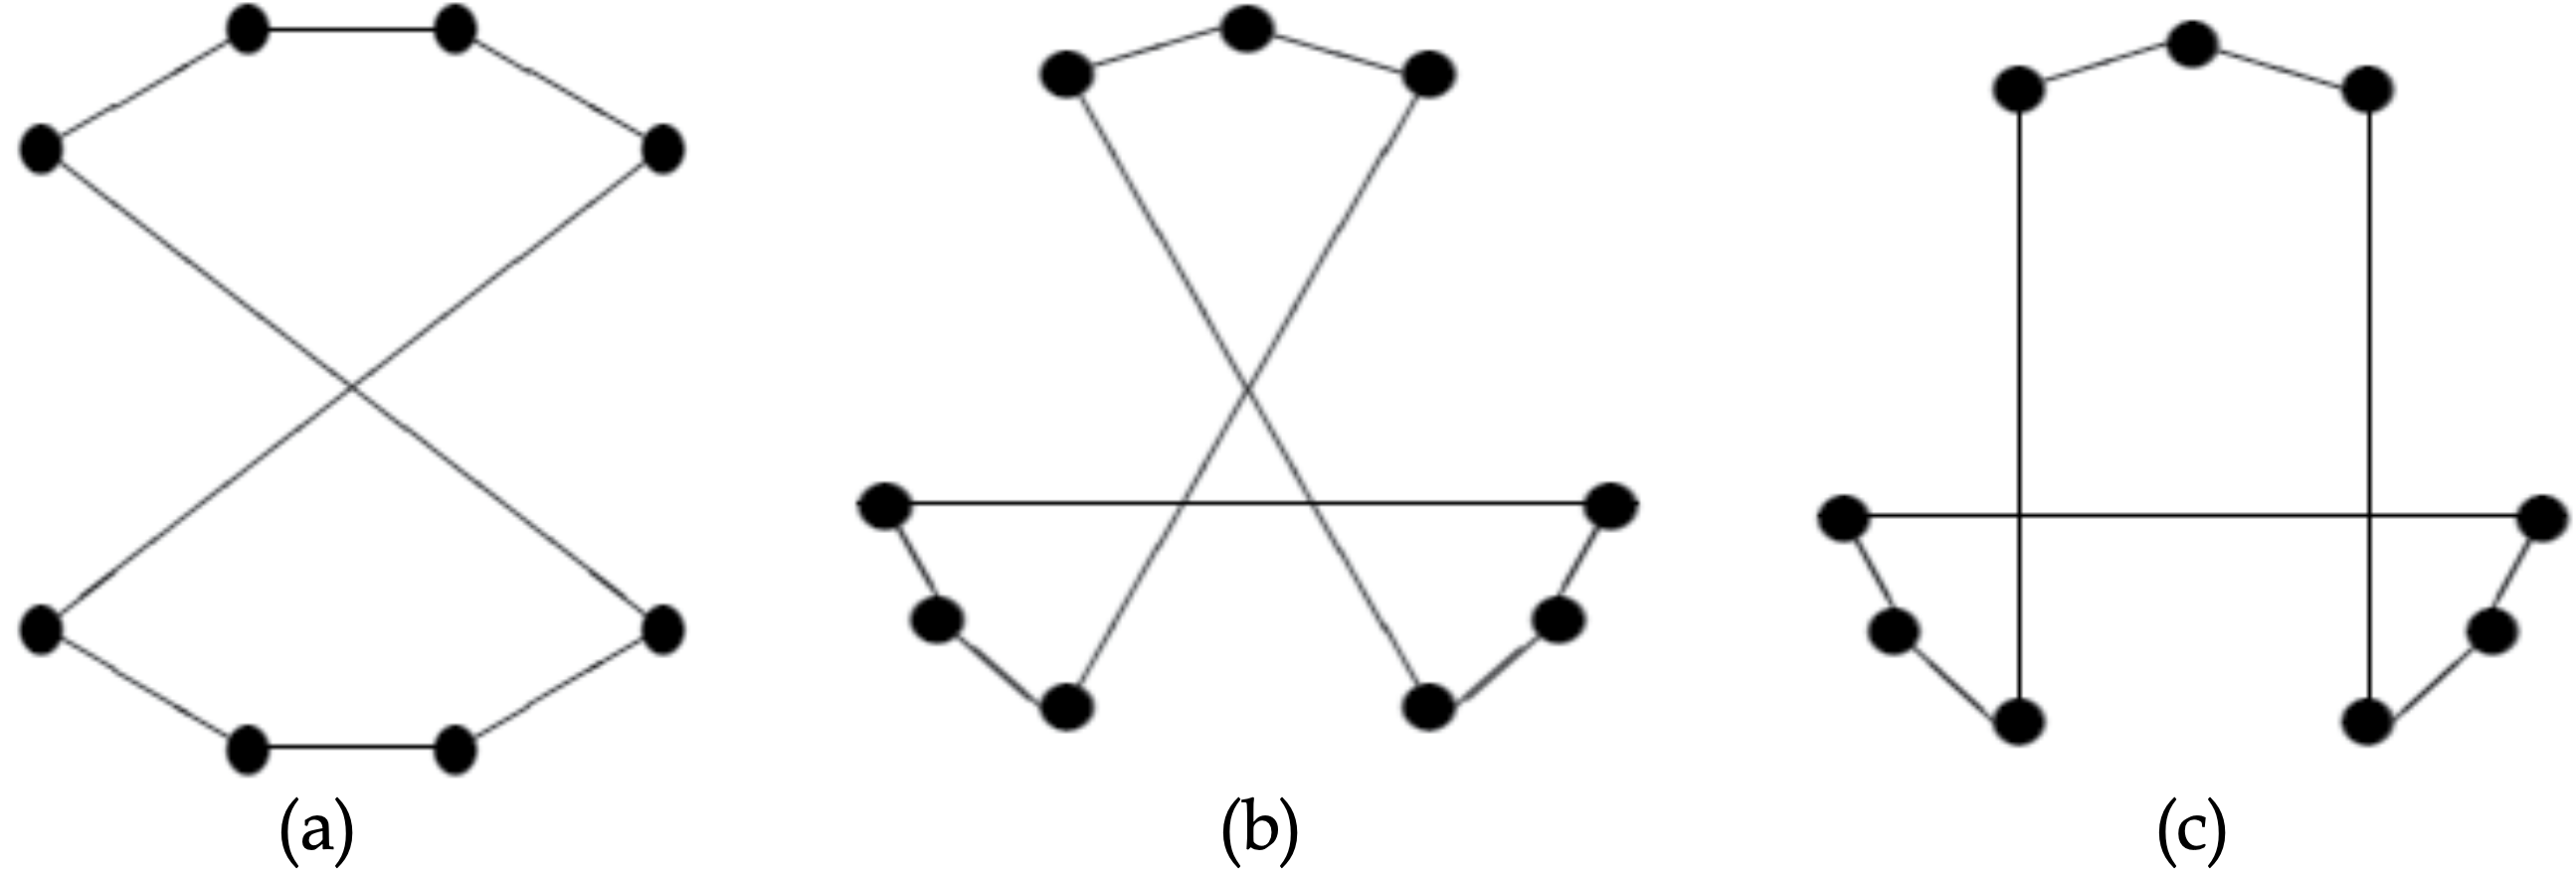
\includegraphics[width=12 cm]{imatges/2-opt_3-opt.png}
  \caption{\label{fig:2opt3opt} Moviment 2-opt i 3-opt}
\end{figure}

\subsubsection{Lin-Kernighan}
\label{LinKernighan}
Lin \& Kernighan van construir un algoritme que fa possible arribar al 2\% del límit inferior de Held-Karp. L'heurística Lin-Kernighan (LK) és una heurística d'intercanvi variable k-way. Decideix el valor de k adequat a cada iteració. Això fa que l'heurística de millora sigui força complexa, i pocs han aconseguit millorar-la. La complexitat temporal de LK és aproximadament \( O(n^{2.2}) \) (Helsgaun), fent que sigui més lenta que una implementació senzilla de 2-opt.

\section{Implementació d'heurístics clàssics}
\label{ImplementacioHeuristicsClassiques}
Les solucions heurístiques clàssiques constitueixen una referència molt útil per a l’avaluació de la xarxa neuronal gràfica que es desenvoluparà més endavant. Per aquest motiu, s’han implementat els algorismes de construcció i millora de circuits descrits anteriorment, que representen alguns dels enfocaments clàssics més utilitzats en la resolució del TSP.

\medskip

El dataset (que es descriurà amb més detall més endavant) inclou, per a cada nombre de vèrtexs (10, 20, 30, 50 i 100), 10.000 grafs generats per a ser utilitzats com a test. Els vèrtexs de cada graf es distribueixen uniformement dins del quadrat unitat, de manera que les coordenades de cada node es troben dins de l’interval $[0,1]^2$. Per a cada graf, el dataset proporciona la seva solució òptima la qual ha estat generada utilitzant el Concorde TSP Solver\cite{ConcordeTSP}.

\medskip

L'avaluació dels models s'efectua comparant la llargada del circuit de la solució generada per cada heurístia amb la llargada del circuit de la solució òptima. La mètrica utilitzada s'anomena \textit{GAP} i es calcula com:
\begin{equation}
  \text{GAP} = \frac{L_{\text{heurístic}} - L_{\text{òptima}}}{L_{\text{òptima}}}
  \label{equ:GAP}
\end{equation}
de manera que un GAP de 0 indica que la solució generada per l'heurístic és òptima. El GAP es pot interpretar com la proporció de com de pitjor és l'heurístic respecte l'òptima.

\medskip

A continuació es presenten els resultats obtinguts per als heurístics de construcció de circuits (Closest Neighbor i Greedy):

\begin{table}[htb]
  \centering
  \begin{tabular}{ | r | c | c | }
   \hline
   \textbf{Nº de vèrtex} & \textbf{Closest Neighbor} & \textbf{Greedy} \\
   \hline
   \textbf{10}  &  &  \\
   \textbf{20}  &  &  \\
   \textbf{30}  &  &  \\
   \textbf{50}  &  &  \\
   \textbf{100} &  &  \\
   \hline
  \end{tabular}
  \caption{Resultats dels heurístics de construcció.}
  \label{taula:heuristicsConstruccio}
\end{table}

\medskip

Per a avaluar el rendiment dels algoritmes heurístics de millora de circuits (2-opt, 3-opt i Lin-Kernighan), s'han aplicat als circuits generats per l'heurístic Closest Neighbor (CN). Els resultats obtinguts es presenten a continuació:

\begin{table}[htb]
  \centering
  \begin{tabular}{ | r | c | c | c | }
   \hline
   \textbf{Nº de vèrtex} & \textbf{CN + 2-opt} & \textbf{CN + 3-opt} & \textbf{CN + Lin-Kernighan} \\
   \hline
   \textbf{10}  &  &  &  \\
   \textbf{20}  &  &  &  \\
   \textbf{30}  &  &  &  \\
   \textbf{50}  &  &  &  \\
   \textbf{100} &  &  &  \\
   \hline
  \end{tabular}
  \caption{Resultats dels heurístics de millora.}
  \label{taula:heuristicsMillora}
\end{table}

\medskip

A continuació es poden visualitzar alguns dels circuits generats pels diferents heurístics:



  

















\newpage





















Aquest és un gran treball que bla, bla, bla,\ldots

Com s'explicarà al Capítol~\ref{cap:prelim} (això és un exemple de referència),\ldots

Això és un exemple de citació d'un llibre~\cite{Coleman1974}, un article científic~\cite{Ruiz2008} i una referència a una web~\cite{Halcon}.

Exemple de taula:
\begin{table}[htb]
\centering
\begin{tabular}{ | r | c | c | l | }
 \hline
  Any & Matriculats & Aprovats & Percentatge\\
\hline
 2019  & 65 & 47 & 72.3\%\\
 2020  & 69 & 48 & 69.6\%\\
 2021  & 75 & 58 & 77.3\%\\
  \hline
  \end{tabular}
\caption{Aquí és on s'ha de posar el peu de taula.}
\label{taula:taulaexemple} 
\end{table}

Exemple de figura:
\begin{figure}[htb]
\centering

\includegraphics[width=8 cm]{imatges/logo_eps.png}
\caption{\label{fig:logo} Logotip de l'Escola Politècnica Superior.}
\end{figure}

Exemple de fòrmula:
\begin{equation}
H(X) = -\sum_{i=1}^{N}p_s(x_i) \log \left( p_s(x_i) \right).
\label{equ:entropia}
\end{equation}


També es pot fer referència en el text a les taules (p.ex. veure la Taula~\ref{taula:taulaexemple}), a les figures (p.ex. veure la Figura~\ref{fig:logo}) o a les fòrmules (p.ex. veure Equació~\ref{equ:entropia}).

Lorem ipsum dolor sit amet, consectetur adipiscing elit. Nunc congue mattis tellus, in rhoncus nisl laoreet vel. Sed nulla libero, tincidunt id ligula congue, hendrerit maximus mi. Morbi nec metus in urna imperdiet mattis pretium a libero. Fusce est mauris, convallis id facilisis faucibus, consequat aliquet eros. Vivamus et dui pulvinar, rutrum velit at, volutpat tellus. Nulla vehicula ullamcorper justo, blandit interdum leo sagittis quis. Quisque convallis vel ante ac rutrum. Morbi et varius sem, sed tristique elit. Vestibulum aliquam facilisis pellentesque. Suspendisse consequat commodo eros, sit amet tincidunt sapien semper in. Nunc ut magna ac quam tempor malesuada et at ex. Donec mattis mauris ante, id condimentum elit dapibus at.

Curabitur ut sodales sapien. Etiam eget ultrices risus, in dignissim nunc. Quisque quis tortor in nunc posuere lacinia ut sed dui. Praesent ut sollicitudin diam, ut mattis magna. Morbi porttitor fermentum magna a pharetra. Nullam at magna diam. Suspendisse vehicula tellus eget ligula aliquam semper. Integer sed ullamcorper felis, ac imperdiet elit. Praesent eu suscipit ligula, sit amet vulputate erat. Etiam eget tempor est, vitae aliquet tortor. Nam efficitur tristique ligula. Aliquam blandit leo non ante suscipit, vitae mattis diam rhoncus. Ut ac dui sit amet dui venenatis suscipit.

Nunc sollicitudin hendrerit risus, quis ultricies orci elementum non. Aliquam erat volutpat. Mauris neque turpis, molestie in tellus id, pharetra gravida mi. Suspendisse potenti. Donec aliquam dolor eu pellentesque auctor. Proin eget sapien ut tellus maximus lacinia. Praesent blandit pretium mi, suscipit sollicitudin eros iaculis in. Nunc a justo sit amet mauris auctor posuere sit amet vel erat. Etiam in maximus nisi. Pellentesque blandit pharetra lectus nec efficitur. Praesent tristique vel arcu id bibendum. In eget eros fringilla magna hendrerit facilisis ac vitae urna. Donec malesuada fermentum dictum. Pellentesque aliquet tortor vitae suscipit tempus. Phasellus ornare risus mi, vel placerat justo efficitur eu. Phasellus quis tincidunt enim.

Etiam a elementum lorem. Integer ac lectus hendrerit, venenatis ante vitae, accumsan eros. Orci varius natoque penatibus et magnis dis parturient montes, nascetur ridiculus mus. Curabitur non varius dolor. Donec suscipit metus vitae ultrices sagittis. Praesent ac dapibus justo, vel mollis sapien. Pellentesque at iaculis neque. Donec ac tellus orci. Pellentesque eleifend fringilla massa, in lobortis nibh finibus in. Morbi ut neque vitae est congue tempor efficitur imperdiet dolor. Pellentesque nec nibh nec nibh fringilla laoreet. Duis fermentum ornare sollicitudin. Maecenas finibus tincidunt justo commodo commodo. Suspendisse venenatis odio dignissim auctor elementum. Duis non mauris orci.



\chapter{Preliminars}
\label{cap:prelim}

\section{Formulació matemàtica del TSP}
\label{Formulacio}

El TSP es pot definir sobre un graf complet no dirigit \( G = (V, E) \) en el cas del sTSP, o sobre un graf dirigit \( G = (V, A) \) en el cas del aTSP.

\begin{itemize}
  \item \( V = \{1, \dots, n\} \) és el conjunt de vèrtexs.
  \item \( E = \{ (i,j) : i,j \in V, i \neq j \} \) és el conjunt d'arestes i \( A = \{ (i,j) : i,j \in V, i \neq j \} \) el conjunt d'arcs.
  \item Es defineix una matriu de costos \( C = \{c_{ij}\} \) sobre \( E \) o \( A \). La matriu de costos compleix la desigualtat triangular sempre que \( c_{ij} \leq c_{ik} + c_{kj} \), per a tots \( i, j, k \). En particular, aquest és el cas dels problemes al pla, en què els vèrtexs són punts \( (X_i, Y_i) \) al pla, i \( c_{ij} = \sqrt{(X_i - X_j)^2 + (Y_i - Y_j)^2} \) és la distància euclidiana. La desigualtat triangular també es compleix si \( c_{ij} \) és la longitud del camí més curt des de \( i \) fins a \( j \) sobre \( G \).
\end{itemize}

\subsection{Formulació del sTSP}
\label{FormulacioSTSP}
La formulació proposada per Dantzig, Fulkerson i Johnson (1954) és una de les formulacions matemàtiques del sTSP més citades. Aquesta formulació associa una variable binària \(x_{ij}\) a cada aresta \( (i,j) \), que pren el valor 1 si i només si l'aresta forma part del circuit òptim. La formulació del sTSP és la següent:

Minimitzar
\begin{equation}
  \sum_{i<j} c_{ij} x_{ij}
  \label{equ:TSP1}
\end{equation}
Subjecte a
\begin{equation}
  \sum_{i < k} x_{ik} + \sum_{j > k} x_{kj}= 2 \quad\quad \left( k \in V \right)
  \label{equ:TSP2}
\end{equation}
\begin{equation}
  \sum_{i, j \in S} x_{ij} \leq |S| - 1 \quad\quad \left( S \subset V, 3 \leq |S| \leq n-3 \right)
  \label{equ:TSP3}
\end{equation}
\begin{equation}
  x_{ij} = 0 \text{ o } 1 \quad\quad (i,j) \in E
  \label{equ:TSP4}
\end{equation}
En aquesta formulació, les restriccions \eqref{equ:TSP2}, \eqref{equ:TSP3} i \eqref{equ:TSP4} s'anomenen restriccions de grau, restriccions d'eliminació de subcicles i restriccions d'integritat, respectivament.

\subsection{Formulació del aTSP}
\label{FormulacioATSP}
La formulació de Dantzig, Fulkerson i Johnson (1954) s'extén fàcilment al cas asimètric. En aquest cas \(x_{ij}\) és una variable binària associada a l'arc \( (i,j) \), que pren el valor 1 si i només si l'arc forma part del circuit òptim. La formulació del sTSP és la següent:

Minimitzar
\begin{equation}
  \sum_{i \neq j} c_{ij} x_{ij}
  \label{equ:TSP5}
\end{equation}
Subjecte a
\begin{equation}
  \sum_{j=1}^{n} x_{ij} = 1 \quad\quad \left( i \in V, i \neq j \right)
  \label{equ:TSP6}
\end{equation}
\begin{equation}
  \sum_{i=1}^{n} x_{ij} = 1 \quad\quad \left( j \in V, j \neq i \right)
  \label{equ:TSP7}
\end{equation}
\begin{equation}
  \sum_{i, j \in S} x_{ij} \leq |S| - 1 \quad\quad \left( S \subset V, 2 \leq |S| \leq n-2 \right)
  \label{equ:TSP8}
\end{equation}
\begin{equation}
  x_{ij} = 0 \text{ o } 1 \quad\quad (i,j) \in A
  \label{equ:TSP9}
\end{equation}


\chapter{Planificació i Metodologia}
\label{cap:plan}

\chapter{Contribució Metodològica}
\label{cap:contrib}

\chapter{Resultats}
\label{cap:result}

\chapter{Conclusions i treball futur}
\label{cap:concl}

\backmatter

%\appendix

%\include{Appendix1}

\bibliographystyle{ThesisStyleBreakable}
\bibliography{biblio}

%\printnomenclature

\end{document}
